
\chapter{Introduction}\label{sec:intro}
%\addcontentsline{toc}{chapter}{\nameref{sec:intro}}
% \vspace{0.5cm}
% \chapterprecishere{``Any finite number divided by infinity is as near to nothing as makes no odds, so the average population of all the planets in the Universe can be said to be zero. From this it follows that the population of the whole Universe is also zero, and that any people you may meet from time to time are merely the products of a deranged imagination.''\par\raggedleft--- \textup{Douglas Adams}, The Restaurant at the End of the Universe}

% \vspace{0.5cm}

Exoplanets orbit stars other than the Sun. Over the past two decades since the first was discovered, new types of exoplanet have been discovered unlike anything in the Solar System. Tidally locked planets, where the same side of the planet always faces its star, are among the most striking examples. The global circulation of an atmosphere that is only heated on one side is very different to anything seen in the Solar System. This thesis considers the formation and behaviour of this global circulation, and investigates a case study of an observed tidally locked terrestrial planet.

Tidally locked planets appear to be common despite their unusual behaviour. Figure \ref{fig:tide-locked-population} shows the exoplanets listed on the NASA Exoplanet Archive\footnote{\url{exoplanetarchive.ipac.caltech.edu}} at the time of writing plotted by stellar masses and semi-major axes. All the planets below the line were estimated to be tidally locked by the simple estimate in \citet{pierrehumbert2018review}. These planets are also generally more easily characterised due to their proximity to their host stars \citep{crossfield2015observations}. This may have created a detection bias, where we are more likely to find tidally locked planets. However, it means that they make up many of the best observational targets, so a theoretical understanding of them will be vital to making the most of upcoming measurements.

% \clearpage
\begin{figure}
  \centering
    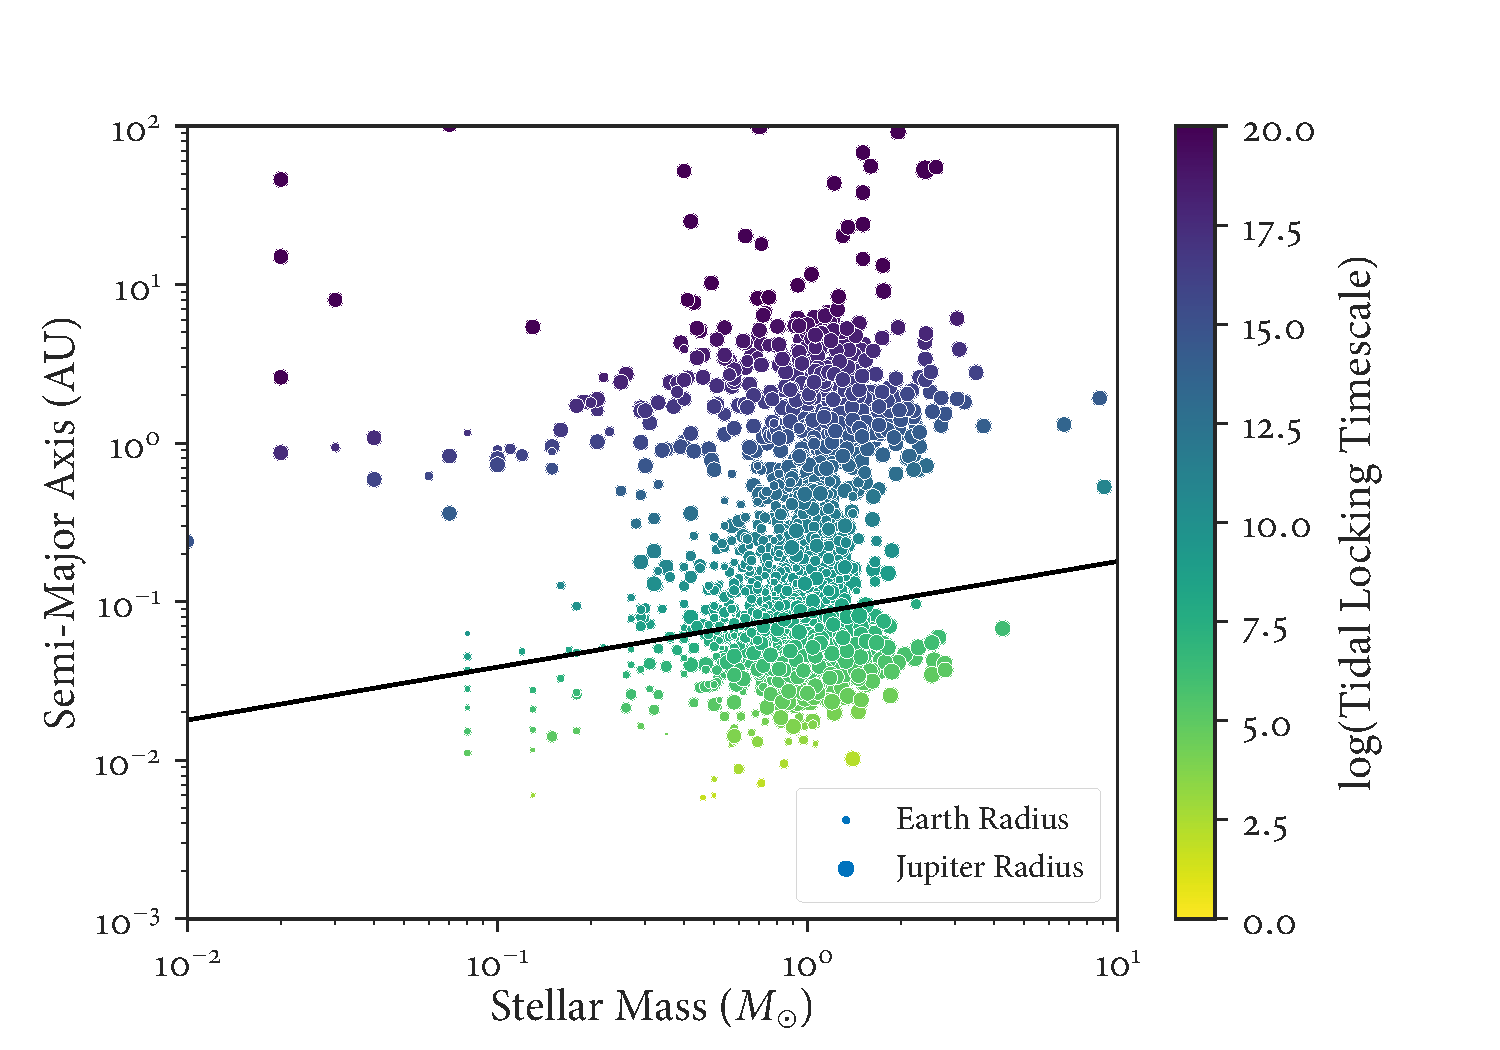
\includegraphics[width=1.0\textwidth]{figures/introduction/tide-locked-population.pdf}
    \caption{The population of known exoplanets plotted by semi-major axis and stellar mass. All the planets below the line have a timescale to reach a tidally locked state of less than 0.1 billion years, so are expected to be in this state. Chapter \ref{ch:lava-planets} explains how this timescale is calculated.}\label{fig:tide-locked-population}
\end{figure}
% \clearpage

% This thesis investigates the atmospheric circulation of tidally locked terrestrial planets.

 Current observations and simulations show that these planets have unique atmospheric dynamics, but the mechanisms for the formation of their global circulation and its effects on planetary climate are not fully understood \citep{heng2015review, pierrehumbert2018review}. The circulation governs the temperature structure of the atmosphere, affecting atmospheric stability, observations of composition, and many other important features.

This thesis has two main themes. In the first part, Chapters \ref{ch:eqm-zonal-flow} and \ref{ch:wave-mean-flow} address the theoretical circulation of terrestrial tidally locked planets and its observational consequences. In the second part, Chapters \ref{ch:linking-climate-55cnce} and \ref{ch:clouds-lava-planets} apply this theory to a case study of the ``lava planet'' 55 Cancri e, using a variety of models to interpret observations of its thermal emission.

The two themes of the thesis are reviewed in Chapter \ref{ch:lava-planets}, ``The Atmospheric Circulation of Tidally Locked Exoplanets'', which discusses relevant work on the subject of tidally locked exoplanets, focusing on the tidal locking process and the resulting atmospheric circulation. It introduces the planet 55 Cancri e, and discusses its observational characterisation to date.

In Chapter \ref{ch:eqm-zonal-flow}, ``The Gierasch-Rossow-Williams Mechanism on Tidally Locked Planets'', I propose a mechanism for the formation of the zonal flow on tidally locked planets. It shows that the meridional circulation is vital to this flow, and uses the equilibrium angular momentum fluxes predicted by the mechanism to explain the behaviour of a suite of atmospheric simulations.

Chapter \ref{ch:wave-mean-flow}, ``Wave-Mean Flow Interactions in Tidally Locked Atmospheres'', is based on \citet{hammond2018wavemean}. I linearise the shallow-water model of \citet{showman2011superrotation} about the equatorial jet discussed in Chapter \ref{ch:eqm-zonal-flow}, and show how the response to stationary forcing explains the form of the global circulation in GCM simulations. This shows that the ``hot-spot shift'' is a result of the interaction of forced stationary waves with the zonal flow, rather than simple advection of heat by the zonal flow.

Chapter \ref{ch:linking-climate-55cnce}, ``Linking the Climate and Thermal Phase Curve of 55 Cancri e'', is adapted from \citet{hammond2017climate}. It compares simulations of the atmosphere of the tidally locked planet 55 Cancri e to the observations of \citet{demory201655cnce}, to constrain the properties of the atmosphere. The observed day-night contrast can be matched with one set of parameters, and the observed hot-spot shift can be matched with another simulation. It is only possible to match the observations completely by adding an estimate of the effect of night-side cloud formation.

In Chapter \ref{ch:clouds-lava-planets}, ``Phase-Resolved Emission Spectra of Potential Climates on 55 Cancri e'', I use an improved model with more realistic radiative transfer to follow up the work in Chapter \ref{ch:linking-climate-55cnce}. The new realistic simulations still obey the scaling relations in Chapter \ref{ch:linking-climate-55cnce}, and are qualitatively similar to the simulation results in the idealised grey-gas model. I show that the simulations with surface pressures of 10 bar do not have phase shifts in their thermal emission at any wavelength, but that a simulation with a surface pressure of 100 bar does have an observable hot-spot shift. I suggest that terrestrial atmospheres with a hot-spot shift will not have a peak offset in their thermal phase curve, unless their atmospheres are sufficiently thick. The chapter concludes that the hot-spot shift observed by \citet{demory201655cnce} is evidence for an atmosphere thicker than 10 bar and with a higher molecular weight than H$_{2}$.

The conclusions in Chapter \ref{ch:conclusions} summarise the results of each chapter, and discuss their significance and the possibility of further work. The first part of the thesis shows how the global circulation of tidally locked planets is governed by their meridional circulation and the stationary waves produced by day-night forcing. I will conclude that the shallow-water models of the formation of zonal flow and a hot-spot shift on a tidally locked planet match GCM simulations, and suggest how the predictions of these models could be tested by observations. The second part of the thesis shows that the observed thermal phase curve of 55 Cancri e is evidence for a thick atmosphere with a surface pressure over 10 bar, with a mean molecular weight greater than H$_{2}$. I will conclude that this thesis has produced a consistent description of the formation of the global circulation of tidally locked terrestrial planets, and suggest future directions for modelling and observations.



% \bibliographystyle{unsrtnat}
% \bibliography{../references.bib}
